% Arna Hyvärinen (updated by Jouni Sampo, 8.10.2024)
% A short example for LaTeX, made with LaTeX

% The idea of this guide is to show how LaTeX code and the resulting document correlate. The idea is to view the code and the document side by side. So, bring up the document now if you haven't already done so.

% Text following the percent symbol is a comment. These are only visible to people reading the code; the machine does not process them.

% These lines define what kind of document this is and how it is formatted. They specify the paper size, font, language, etc.
% The following settings are suitable for reports. Other document styles can be found in the guide -> http://tug.ctan.org/info/lshort/finnish/lyhyt2e.pdf
% This guide will be referenced later as well. It's worth taking a look.

\documentclass[12pt, titlepage, a4paper]{article}  % 12pt is the font size, which can be changed here.

% usepackages are like subroutine libraries. They allow you to use new functionalities that are not included in the basic versions. If a feature doesn’t work but the code is correct, check if the appropriate usepackage is included.

% Below are packages related to the character set being used. The choice depends a bit on the environment and what special characters (e.g., umlauts) you want to write directly from the keyboard.
\usepackage[utf8]{inputenc} % This makes umlauts work, e.g., on  "overleaf.com"
%  online environment
%\usepackage[latin1]{inputenc}   % A common alternative to the above in many other environments
\usepackage[T1]{fontenc}   % A package related to hyphenation and copy/paste functionality in the final product (pdf). For example, ä is treated as its own symbol and not as "a with two dots."
\usepackage[english]{babel}   % Language. Affects for example that hyphenation is done correctly. 

\usepackage{amssymb,amsmath}    % Handy mathematics library

\usepackage{tikz}    % Enabling the TikZ package, required for images. More about TikZ later.
\newcommand*\circled[1]{\tikz[baseline=(char.base)]{
           \node[shape=circle,draw,inner sep=2pt] (char) {#1};}}
\usetikzlibrary{arrows}
\usetikzlibrary{decorations.pathreplacing}

\usetikzlibrary{fadings}
\tikzfading[name=fade out,
  inner color=transparent!0, outer color=transparent!100]
  
\linespread{1.5}       % Defining line spacing

% The text begins. Any text before this point is an error.

\begin{document}    % This tells LaTeX that the definitions are over, and it is time to compile the text. Any commands before this or after are errors.

\noindent       % No indentation for the new line
Lappeenranta University of Technology \hfill{\today} \\   % Date on the right
Faculty \\
Department \\
Course \\

% Advanced trickery to get the name centered. These don’t need to be understood, just copy them directly.
\vspace*{\stretch{2}}       % The number might need to be adjusted, depending on the number of lines at the top and bottom of the page
\begin{center}
\begin{minipage}{.65\textwidth}    % The decimal might need to be adjusted manually

\Huge{A Short Example for \LaTeX}

\end{minipage}
\end{center}
\vspace{\stretch{3}}

{\hfill Arna Hyv{\"a}rinen \& Jouni Sampo}       % Align to the right

\newpage       % New page

\tableofcontents    % Table of contents. LaTeX automatically detects and arranges the headings and subheadings in the correct order, adds page numbers, and all other nice things that in Word need to be done manually. For comparison, masochists can try to do this in Word; it’s not fun.
% NOTE! The table of contents will not appear the first time the code is run, as LaTeX will only detect the headings after the first run. It will appear after the second run. SO THE CODE MUST BE RUN TWICE.
% (This may not apply to all drivers. In this example, TeXShop has been used as the default driver.)

\newpage

%%%%%%%%%%%%%%%%%%%%%%%%%%%%%%%%%%%
% ABOUT WRITING TEXT IN GENERAL

\section{First Section}

\section{About Writing Text in General}    % Defining the title. This way, LaTeX formats the title properly and notes it for the table of contents.

The idea of this guide is to show how \LaTeX code and the resulting document correlate. The idea is to view the code and document \emph{side by side}. So, bring up the code now if you haven’t already, and look through it up to this point.

Here is where the body text goes. It can be written directly. The number of spaces within the text doesn’t matter, they are all treated as one. \LaTeX is blind to spaces, so you can use tabs in the code however you like. The number of line breaks doesn’t matter either, from two upwards (except in some special environments like align). However, it’s a good idea to keep the code neat and readable, so don’t misuse indentations and comments.

If there’s an error in the code, you’ll get an error message when running it. The error message gives a description of the error and the line where the problem occurred. Based on this, the issue can be fixed.
A new line doesn’t start in the text even if there’s a line break in the code. \\
A new line starts with two backslashes or the newline command. \newline Now the line has changed.

An empty line starts a new paragraph.

\LaTeX contains some special characters. The most important one is the backslash $\backslash$, as it starts all commands. Other characters that cannot be written directly are:

\# \$ \% \^{} \& \_ \{ \} \~{} 

These are included in the text by using a backslash. These characters either have a special meaning in code (e.g., \% is a comment symbol) or cause a font issue.

''Quotation marks'' "work" 'inconsistently.' To get a proper quotation mark in the text, you need to use two single ' marks.
Hyphens, en dashes, and em dashes work on the same principle: - -- ---
Ellipsis requires its own command, called ldots. Compare ... and \ldots

You can also add images to the text. However, they may jump around if there’s not enough space on the page, but you can try to guide \LaTeX.
You can also draw images yourself using TikZ, as shown in the example image. More on this later.

%%%%%%%%%%%%%%%%%%%%%%%%%%%%%%%%%%%
% IMAGE

% Image
\begin{figure}[h!]    % As with text boundaries, image boundaries also need to be defined. The letter in square brackets defines how the image is positioned relative to the text. See http://tex.stackexchange.com/questions/35125/how-to-use-the-placement-options-t-h-with-figures
\vspace{-10 pt}
\begin{center} 
% \includegraphics[width=0.5\textwidth]{Kalastaja.pdf}    % Image width relative to text width, and the name of the image file. The image file must be in the same folder as the code file, or else the path must also be defined.
\end{center} 
\caption{Caption}
\vspace{10 pt}
\end{figure}

It's also good to know about the commands \underline{underline} and \emph{emph}. \emph{Inside the emph command, another emph command makes \emph{normal} text.}

%%%%%%%%%%%%%%%%%%%%%%%%%%%%%%%%%%%
% LISTS

\newpage
There are three types of lists: 
First start with command {\it enumerate}, as an example 

\begin{enumerate}
\item First item
    \begin{enumerate}    % Sub-items can have their own list
    \item sub item
        \begin{enumerate} 
        \item subsub item
        \item another subsub item
        \end{enumerate}
    \end{enumerate}
\item Second item
\end{enumerate}
By default, first level items are numbered in arabic numbers, second level with alphabetic and third level Roman numberign.\\\\
Another usufull list structure star with command {\it enumerate}.

\begin{itemize}
\item item
\item[--] French item
\item[$\heartsuit$] arbitrary item    % You can put whatever you want in square brackets
\end{itemize}
You can create also here sub items.

Last but less used list environment is {\it description}:

\begin{description}
\item[first] item
\item[second] item
\end{description}

The syntax is almost the same for all.

Tables can also be created. The command is tabular. A good way to learn how complex systems work is to take example code and remove or add commands to see what happens. This way, you can deconstruct the code. \newline


%%%%%%%%%%%%%%%%%%%%%%%%%%%%%%%%%%%
% TABLE

\begin{tabular}{| r | l |}     % The first column is aligned to the right (r), the second to the left (l). You could also use c for center. Vertical lines indicate the vertical lines of the table.
\hline    % Horizontal line
7C0 & hexadecimal \\    % & indicates a new cell
3700 & octal \\ \cline{2-2}    % Horizontal line from cell 2 to cell 2
11111000000 & binary \\
\hline \hline    % 2 horizontal lines
1984 & decimal \\
\hline    % Horizontal line
\end{tabular}
\newline

More fancy things needs bit more knowlegde.
For example the command @{,} can replace the column separator with a comma (or any other character). This way, you can create tables where the decimals are aligned.

\begin{tabular}{c r @{,} l}
Pi notation     &
\multicolumn{2}{c}{Value} \\        % Combine the next 2 cells, centering the text
\hline
$\pi$               & 3&1416  \\
$\pi^{\pi}$         & 36&46   \\
$(\pi^{\pi})^{\pi}$ & 80662&7 \\
\end{tabular}

Tables may also float, just like images. These are known as floating elements. Placements work the same way as with images.

\subsection{Subsection}
For demonstration purposes.\footnote{Footnotes are created with the footnote command.}

\subsubsection{Sub-subsection}
You cannot go deeper than this.


%%%%%%%%%%%%%%%%%%%%%%%%%%%%%%%%%%%
% MATHEMATICAL FORMATTING

\section{Mathematical Formatting}

\LaTeX produces beautiful text and tables, but it truly shines when formatting mathematics.

Some described features of the mathematical environment are not available directly; they must be included by adding packages at the beginning of the code. If the compiling gets stuck, even if the command is correct, this is likely the issue.

To insert mathematical text among regular text, place it between two \$ signs: $x$ or $E=mc^{2}$. However, it is better to put equations on their own lines: the commands are displaymath or equation. Using equation, you can refer to an equation (\ref{pythagoras}) neatly with label and ref commands, but just like with the table of contents, this requires two runs. \LaTeX keeps track of everything, so you don't need to worry about the numbers. The equation command numbers the equation even if it is not referenced.

\begin{displaymath}
c^{2}=a^{2}+b^{2}
\end{displaymath}
\begin{equation} \label{pythagoras2}
c^{3}=a^{3}+b^{3} + c^{3}=a^{3}+b^{3}
\end{equation}

\begin{equation} \label{pythagoras}
c^{2}=a^{2}+b^{2}
\end{equation}

\begin{equation} 
c^{2}=a^{2}+b^{2}
\end{equation}

The \$ sign-based mathematical environment behaves differently from the displaymath-type environment: the \$ signs are meant to be used within text, so the text is compressed. Compare

$\lim_{n \to \infty} \sum_{k=1}^n \frac{1}{k_2} = \left( \frac{\pi^2}{6} \right)^2$ \\
and 
\begin{displaymath}
\lim_{n \to \infty} \sum_{k=1}^n \frac{1}{k_2} = \left( \frac{\pi^2}{6} \right)^2
\end{displaymath}

You can also access the displaymath environment using brackets. If you want regular text in a mathematical environment, you can use the \textrm\{\} command:

\[ c^{2}=a^{2}+b^{2} \textrm{ is the Pythagorean theorem.} \]

Formatting commands should generally be placed in curly braces. Compare

\[ a^x+y \textrm{ and } a^{x+y} \]

Different symbols, letters, and formats can be found in the \emph{guide}, Chapter 3. Building equations starts on page 51.

Writing multiple lines can be somewhat clunky with displaymath. A convenient environment is align, which uses the \& sign to align all lines. The align environment with * does not number the lines.

\begin{align*}
f(x) + g(x) &= (4x^3 + 6)+ (6x^4 -x^3 + x^2)\\
&= 6 + (0+0)x+(0+1)x^2 + (4-1)x^3+(0+6)x^4\\
&= \underbrace{6}_{a_0} + \underbrace{0}_{a_1}x + \underbrace{1}_{a_2}x^2 + \underbrace{3}_{a_3}x^3 + \underbrace{6}_{a_4} x^4
\end{align*}

\begin{align}
f(x) + g(x) &= (4x^3 + 6)+ (6x^4 -x^3 + x^2)\\
&= 6 + (0+0)x+(0+1)x^2 + (4-1)x^3+(0+6)x^4\\
&= \underbrace{6}_{a_0} + \underbrace{0}_{a_1}x + \underbrace{1}_{a_2}x^2 + \underbrace{3}_{a_3}x^3 + \underbrace{6}_{a_4} x^4
\end{align}



%%%%%%%%%%%%%%%%%%%%%%%%%%%%%%%%%%%
% USEFUL LINKS

\section{Useful Links}

It is important to remember that \LaTeX is a programming language like any other. You can find guides and solutions to problems by googling.

\begin{itemize}

\item http://tug.ctan.org/info/lshort/english/lshort.pdf
\subitem A guide, but not too deep. IT IS ALLOWED, EVEN PREFERABLE, TO USE GUIDES AND EXAMPLES FOUND ON THE INTERNET.
\item https://www.overleaf.com/
\subitem Another online compiler
\item http://cremeronline.com/LaTeX/minimaltikz.pdf
\subitem A short TikZ guide
    \begin{itemize}
    \item{http://www.texample.net/tikz/examples/}
    \subitem{Examples of all kinds}
    \end{itemize}
\item http://detexify.kirelabs.org/classify.html
\subitem A handy symbol search system
\item http://tug.ctan.org/info/symbols/comprehensive/symbols-a4.pdf
\subitem A list containing \emph{all} symbols, from various euro symbols to Icelandic magical symbols \footnote{Wink wink, investors.}.

\end{itemize}







%%%%%%%%%%%%%%%%%%%%%%%%%%%%%%%%%%%
% OTHER COOL THINGS

\section{Other Stuff}

With these tools, you can get quite far and write all your reports and so on. The following topics are neat and interesting, but you don’t need to know them if you just want to use \LaTeX. Those who are curious can continue from here, while the more relaxed can move on to the exercise.

\subsection{TikZ}

TikZ is a method to draw vector graphics. The aforementioned TikZ guide is quite competent, though very minimalist (as the title suggests). It gets you off to a good start, but you’ll find new tricks by searching. It’s recommended to deconstruct various examples.

% Image
\begin{figure}[h!]
\begin{center}
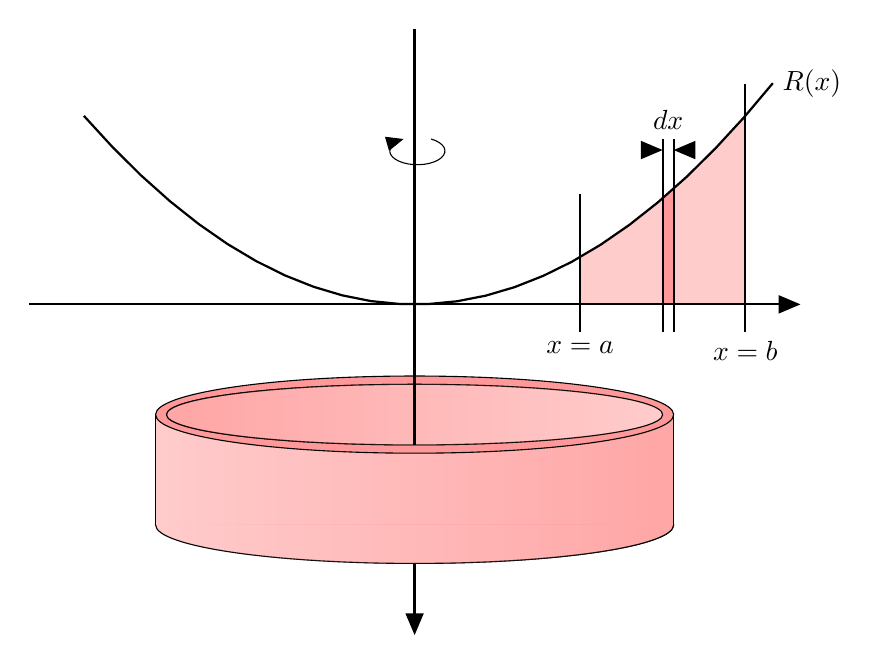
\begin{tikzpicture}[scale=0.7]

\fill[fill=white!80!red] (3,0)--plot [domain=3:6] (\x, {0.095*(\x)^2})--(6,0);
\fill[fill=white!60!red] (4.5,0)--plot [domain=4.5:4.7] (\x, {0.095*(\x)^2})--(4.7,0);

\draw [thick] (6,-0.5)--(6,4);
\draw [thick] (3,-0.5)--(3,2);

\draw [thick, domain=-6:6.5] plot (\x, {0.095*(\x)^2});

\draw [-triangle 45, rotate=-90] (-3,0.3) arc[x radius = 0.25cm, y radius=0.5cm, start angle=150, end angle = -150];

\draw [thick] (4.5,-0.5)--(4.5,3);
\draw [thick] (4.7,-0.5)--(4.7,3);

\draw [thick, -triangle 45] (4.4,2.8)--(4.5,2.8);
\draw [thick, -triangle 45] (4.9,2.8)--(4.7,2.8);

\draw [thick, -triangle 45] (-7,0)--(7,0);
\draw [thick, -triangle 45] (0,-4.7)--(0,-6);

\node at (6.5,4) [right] {$\large R(x)$};
\node at (4.6,3) [above] {$\large dx$};
\node at (3,-0.5) [below] {$x=a$};
\node at (6,-0.5) [below] {$x=b$};

% Ring
\draw [fill=white!80!red,] (0,-4) ellipse (4.7cm and 0.7cm);
\draw [fill=white!65!red, path fading=west] (0,-4) ellipse (4.7cm and 0.7cm);

\draw [white!80!red, fill=white!80!red](-4.7,-4) rectangle (4.7,-2);
\draw [white!65!red, fill=white!65!red, path fading=west](-4.7,-4) rectangle (4.7,-2);
\draw (4.7,-2)--(4.7,-4);
\draw (-4.7,-2)--(-4.7,-4);

\draw [fill=white!60!red] (0,-2) ellipse (4.7cm and 0.7cm);

\draw [fill=white!80!red] (0,-2) ellipse (4.5cm and 0.55cm);
\draw [fill=white!65!red, path fading=east] (0,-2) ellipse (4.5cm and 0.55cm);

\draw [thick] (0,5)--(0,-2.55); % axis in between

%\draw [help lines] (-6,-7) grid (10,5);

\end{tikzpicture}
\end{center}
\caption{A skilled creator can make all kinds of cool things.}
\end{figure}

% Image
\begin{figure}[h!]
\begin{center}
\begin{tikzpicture}

\begin{scope}[scale=1.75]
  \foreach \c [count=\i from 0] in {red!75!black}{

    \tikzset{xshift={mod(\i,2)*3cm}, yshift=-floor(\i/2)*3cm}
    \colorlet{cup}{\c}

    % Saucer
    \begin{scope}[shift={(0,-1-1/16)}]
      \fill [black!87.5, path fading=fade out] 
        (0,-2/8) ellipse [x radius=6/4, y radius=3/4];
      \fill [cup, postaction={left color=black, right color=white, opacity=1/3}] 
        (0,0) ++(180:5/4) arc (180:360:5/4 and 5/8+1/16);
      \fill [cup, postaction={left color=black!50, right color=white, opacity=1/3}] 
        (0,0) ellipse [x radius=5/4, y radius=5/8];
      \fill [cup, postaction={left color=white, right color=black, opacity=1/3}]
        (0,1/16) ellipse [x radius=5/4/2, y radius=5/8/2];
      \fill [cup, postaction={left color=black, right color=white, opacity=1/3}] 
        (0,0) ellipse [x radius=5/4/2-1/16, y radius=5/8/2-1/16];
    \end{scope} 

    % Handle
    \begin{scope}[shift=(10:7/8), rotate=-30, yslant=1/2, xslant=-1/8]
      \fill [cup, postaction={top color=black, bottom color=white, opacity=1/3}] 
        (0,0) arc (130:-100:3/8 and 1/2) -- ++(0,1/4) arc (-100:130:1/8 and 1/4)
        -- cycle;
      \fill [cup, postaction={top color=white, bottom color=black, opacity=1/3}] 
        (0,0) arc (130:-100:3/8 and 1/2) -- ++(0,1/32) arc (-100:130:1/4 and 1/3)
        -- cycle;
    \end{scope}

    % Cup
    \fill [cup!25!black, path fading=fade out] 
      (0,-1-1/16) ellipse [x radius=3/4, y radius=1/3];
    \fill [cup, postaction={left color=black, right color=white, opacity=1/3/2},
      postaction={bottom color=black, top color=white, opacity=1/3/2}] 
      (-1,0) arc (180:360:1 and 5/4);
    \fill [cup, postaction={left color=white, right color=black, opacity=1/3}] 
      (0,0) ellipse [x radius=1, y radius=1/2];
    \fill [cup, postaction={left color=black, right color=white, opacity=1/3/2},
      postaction={bottom color=black, top color=white, opacity=1/3/2}] 
      (0,0) ellipse [x radius=1-1/16, y radius=1/2-1/16];

    % Coffee
    \begin{scope}
      \clip ellipse [x radius=1-1/16, y radius=1/2-1/16];
      \fill [brown!25!black] 
        (0,-1/4) ellipse [x radius=3/4, y radius=3/8];
      \fill [brown!50!black, path fading=fade out] 
        (0,-1/4) ellipse [x radius=3/4, y radius=3/8];
    \end{scope}
  }
  
\end{scope}
  
\end{tikzpicture}
\end{center}
\caption{Necessary and unnecessary things.}
\end{figure}

\subsection{BibTeX}

The idea of BibTeX is to automate citation making. In longer academic writings (e.g., dissertations), there are a lot of citations. With an automatic system, citations remain uniform and well-organized.

The command is \cite{referenceID}. \cite{bar}

BibTeX is automatically included in \LaTeX's standard distribution, so it does not need to be downloaded separately. However, some formatting styles may require additional usepackage commands to access them.

The most challenging part is creating the bibliography. One way to do this is to open a new file in TeXShop, place the bibliography code there, and save it directly in bib format. To include references in the code, it needs to be run multiple times again. Depending on how the bib bibliography is created, the code sometimes needs to be run in BibTeX format (in TeXShop, this can be done using the dropdown menu next to the Typeset button) and then a couple more times in LaTeX format. The bibliography file must be in the same directory as the other code.

The library can also be edited (or created) using the BibDesk utility. It should be included in the standard TeXShop distribution. The code-level bibbing can be found in the guide.

Guide: https://www.economics.utoronto.ca/osborne/latex/BIBTEX.HTM  
Those interested in the topic should also try Googling it themselves.

Lorem ipsum \cite{ahu61}. \\ % Reference  
Dolor sit amet \cite[p. 2]{bar}  % Reference to page, square brackets can contain anything

\bibliographystyle{amsplain}	% There are various styles; this one is quite good.  
\bibliography{examplebib}	% Which bibliography is this

\end{document}   % The document ends here

This text does not appear, as it is after \end{document}. Any text that comes now is not considered. Formatting commands could theoretically be placed here, but it is very bad style. To obtain clean and readable code, all formatting things should be at the beginning.

%eof		% Writing with LaTeX is coding, and it is good coding practice to mark when the code ends. This way, there won't be any surprises after a dozen empty lines. Comamand on line 428 should typically be the 

